\documentclass[conference]{IEEEtran}
\IEEEoverridecommandlockouts

\usepackage{cite}
\usepackage{amsmath,amssymb,amsfonts}
\usepackage{graphicx}
\usepackage{textcomp}
\usepackage{xcolor}
\usepackage{float}
\usepackage{hyperref}
\usepackage{listings}

\def\BibTeX{{\rm B\kern-.05em{\sc i\kern-.025em b}\kern-.08em
    T\kern-.1667em\lower.7ex\hbox{E}\kern-.125emX}}
\begin{document} 


\title{Design of a Simple CS Amplifier}

\author{\IEEEauthorblockN{Emmanuel Jesus R. Estallo}
\IEEEauthorblockA{\textit{Electrical and Electronics Engineering Institute} \\
\textit{University of the Philippines - Diliman}\\
Quezon City, Philippines\\
emmanuel.estallo@eee.upd.edu.ph}}

\maketitle

\section{CS Amplifier} 
\noindent The desired specs are as follows:
\begin{itemize}
	\item $|A_v|>40$ at $V_{DS}=V_{DD}/2=0.9V$
	\item Output swing: $400mV$
	\item Unity-gain frequency: $f_u=100MHz$, $C_L=5pF$
	\item $V^{*}=200mV$
\end{itemize}
The transconductance can be obtained from:
\begin{equation*}
	g_m = 2\pi f_u C_L
\end{equation*}
this gives us
\begin{equation*}
	g_m = 3.14\; mS
\end{equation*}
The current can be obtained from: 
\begin{equation*}
	V^* = 2\cdot\left( \frac{g_m}{I_D}\right)^{-1} 
\end{equation*} 
and a $V^*$ of $200\; mV$ corresponds to a $g_m/I_D$ of 10. 

\vspace{8pt}
\noindent Thus, 
\begin{equation*}
	I_D = 314\; \mu A
\end{equation*}
The $V^*$ vs $I_D$ plot for a transistor with $W=1\mu m$, $L=0.30 \mu m$ is shown below. 
\begin{figure}[H]
	\centering 
	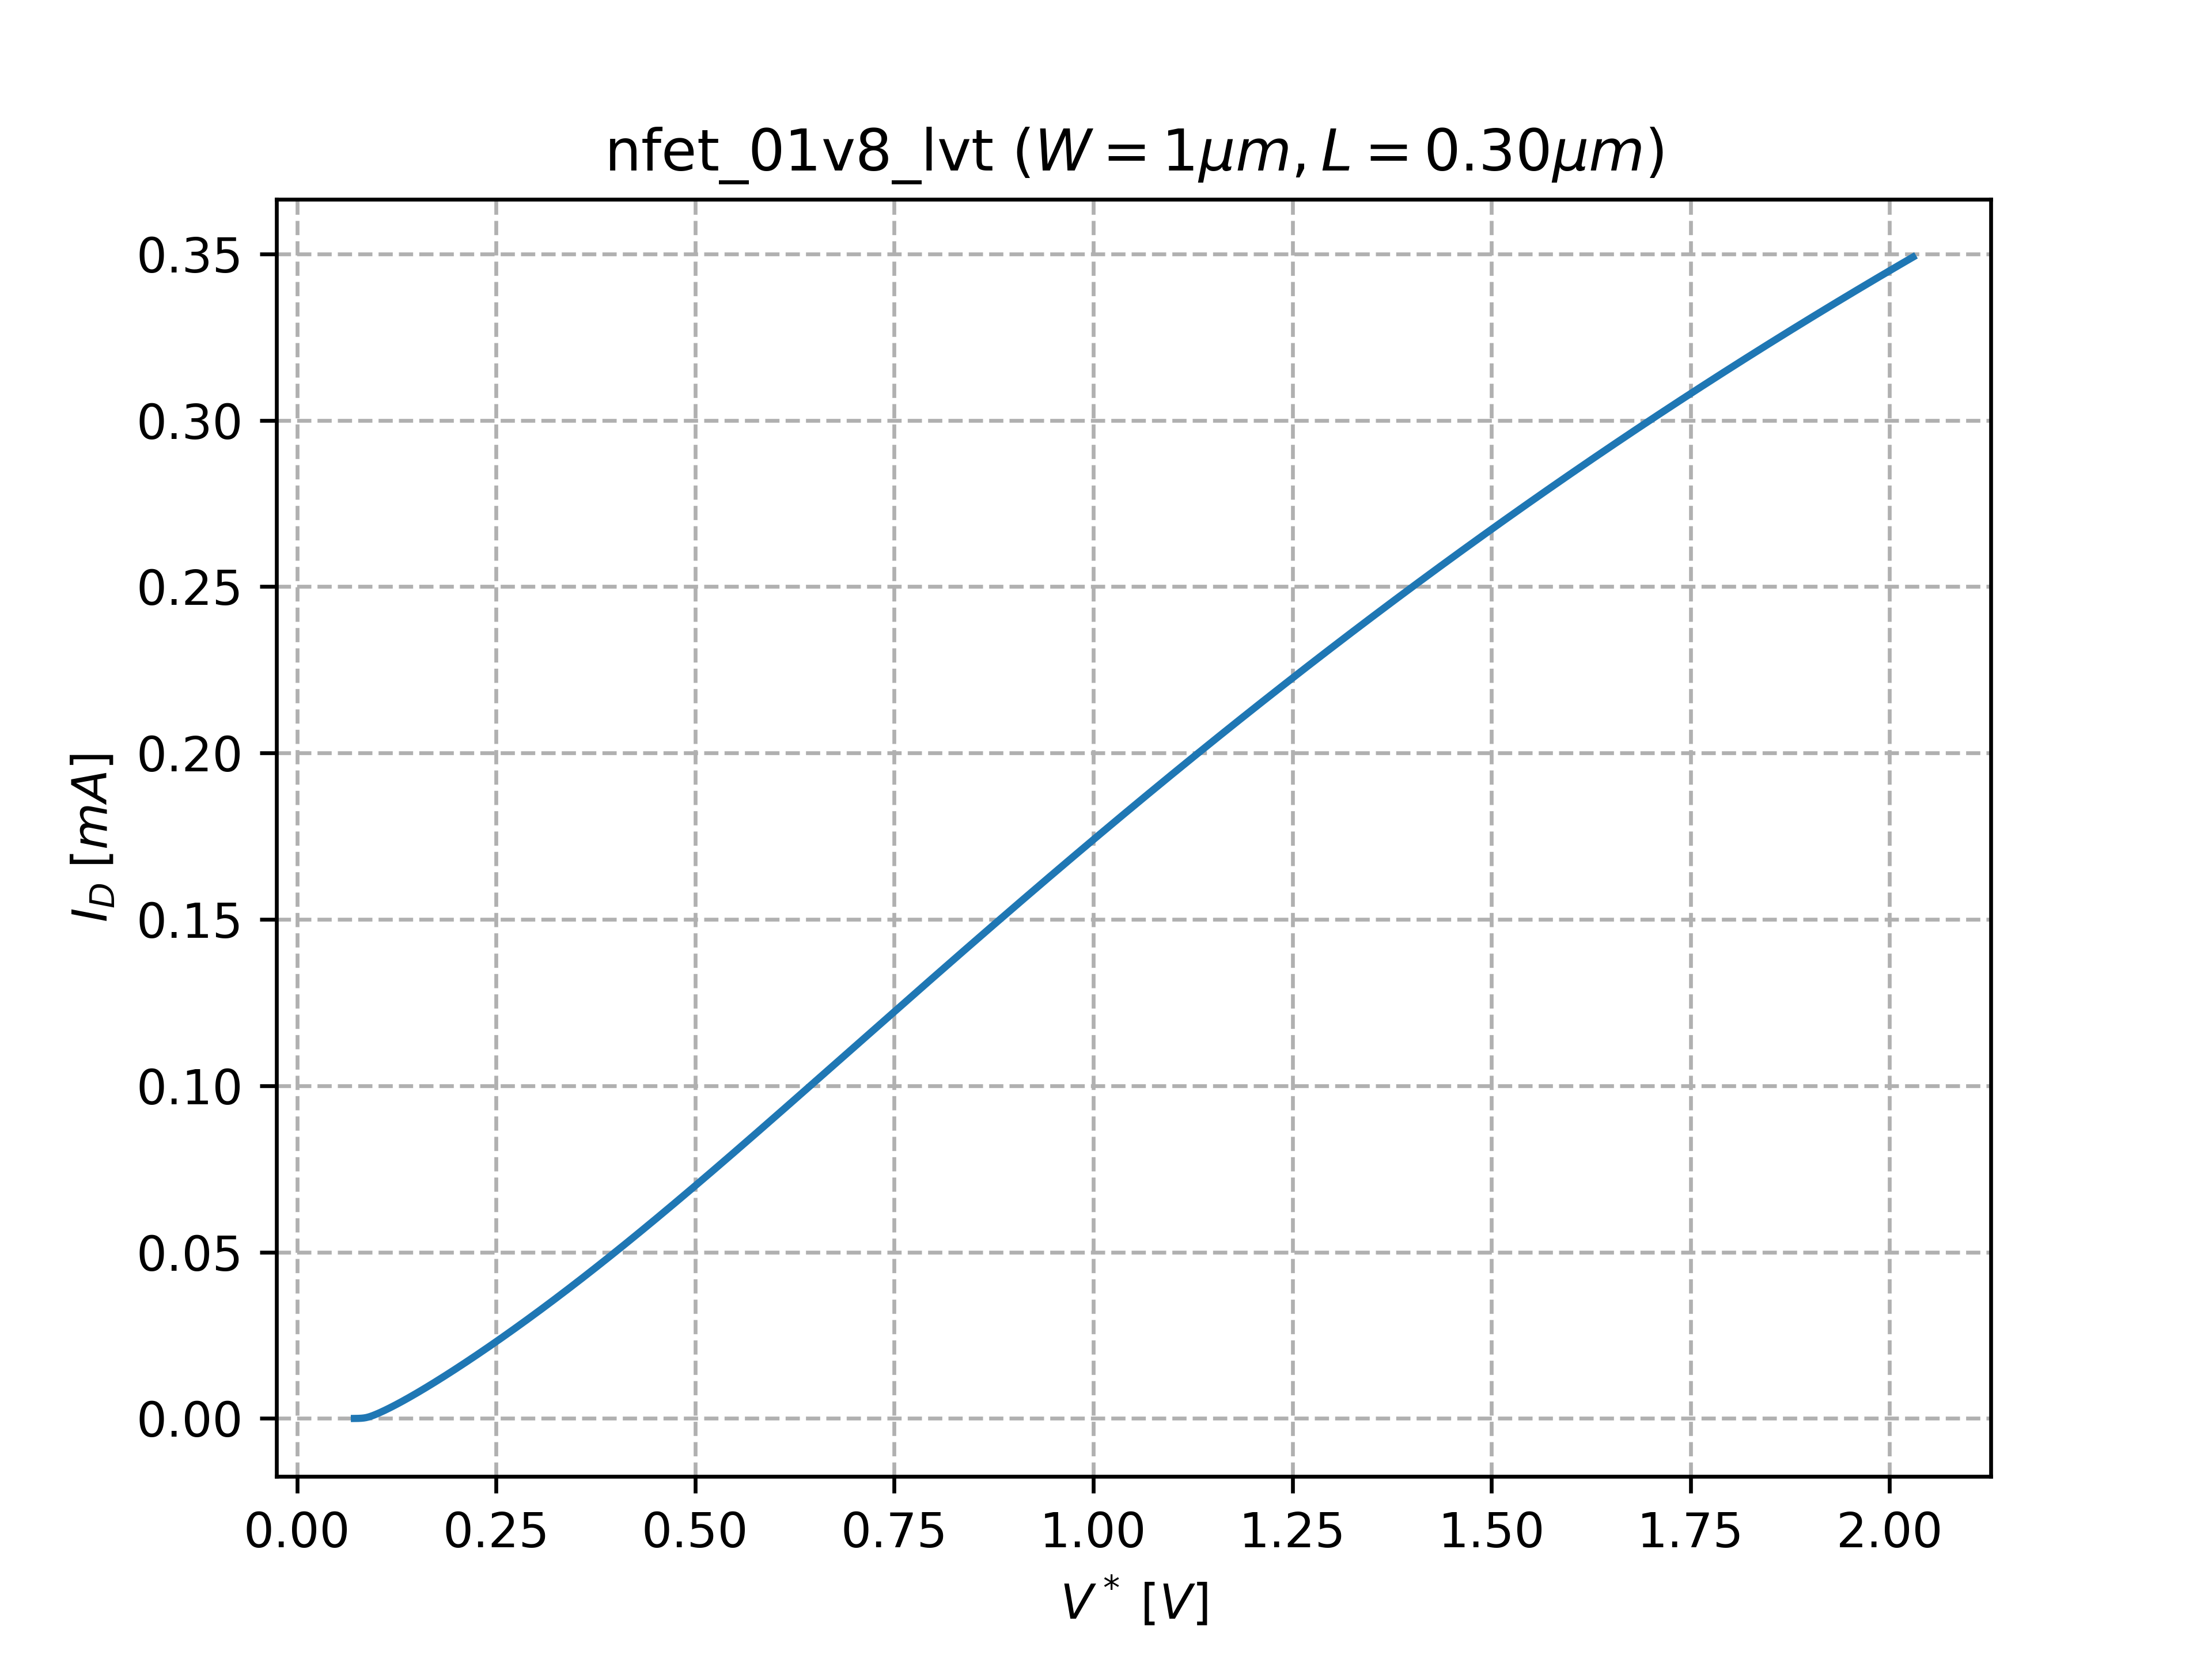
\includegraphics[width=\columnwidth]{vstar-id.png}
	\caption{$I_D$ vs $V^*$}
	\label{vstar-id}
\end{figure}
To get the desired $I_D$, the width should be multiplied by 21. 


\end{document} 
